\documentclass[a4paper,10pt]{article}
%\usepackage[latin1]{inputenc} % Paquetes de idioma
\usepackage[utf8]{inputenc} % Paquetes de idioma (Este encoding toma acentos :) )
\usepackage[spanish]{babel} % Paquetes de idioma
\usepackage{graphicx} % Paquete para ingresar gráficos
\usepackage{grffile}
\usepackage{hyperref}
\usepackage{fancybox}
\usepackage{amsmath}
\usepackage{amsfonts}
\usepackage{listings}
\usepackage{float}
% Paquetes de macros de Circuitos
%\usepackage{pstricks}
\usepackage{tikz}

% Encabezado y Pié de página
\usepackage{fancyhdr} % Paquete para encabezados y pie de página
\pagestyle{fancy} % Sin esta línea no se imprimiría el encabezado en todas las páginas

\fancyhf{} %  Borra el encabezado anterior (Por defecto escribe el títutlo de la sección en la que se encuentra la hoja
\setlength{\headheight}{22.55pt}
\fancyhead[L]{
	{\textsf{Facultad de Ingenier\'ia $-$ Universidad de Buenos Aires \\ 66.44 Instrumentos Electrónicos}}
}
%\addtocounter{page}{5}
\fancyhead[R]{\thepage}

\renewcommand{\footrulewidth}{0.4pt} % Ajusta el tamaño de las líneas separadoras en el pié de página
\renewcommand{\headrulewidth}{0.4pt} % Ajusta el tamaño de las líneas separadoras en el encabezado

\fancyfoot[L]{
	{\textsf{Trabajo Pr\'actico N$^{\circ}4$}: Mediciones de impedancias} \\
	{\textsf{Integrantes: Eduardo Sanchez, Francisco Soler}}
	}
		

% Carátula del Trabajo
\title{ \author{} % Lo pongo para que el warning no moleste :p
\setlength{\unitlength}{1cm} %  Especifica la unidad de trabajo
\thispagestyle{empty}

\begin{picture}(18,0)
\put(0,0){
\includegraphics[width=1.5cm, height=3cm]{Logo1.png}}

\put(10.5,0){
\includegraphics[width=3cm, height=3cm]{Logo2.png}}

\end{picture}
\\[1.5cm]
\begin{center}
	\textbf{{\Huge Facultad de Ingenier\'ia \\ Universidad de Buenos Aires}}\\[2cm]
	{66.44 Instrumentos Electrónicos}\\[0.5cm]
	{Trabajo Pr\'actico N$^{\circ}3$: Mediciones de impedancias}\\[2.5cm]
\end{center}

\begin{flushleft}
	\textbf{Integrantes:} \\[1cm]

	\begin{tabular}{|c|c|c|}
		\hline
		\textbf{\normalsize Padr\'on} & \textbf{\normalsize Nombre} & \textbf{\normalsize Email} \\
		\hline
		\normalsize 92903 & \normalsize Sanchez, Eduardo Hugo & \normalsize hugo\_044@hotmail.com \\
		\hline
		\normalsize 91227 & \normalsize Soler, Jos\'e Francisco & \normalsize francisco.\_tw@hotmail.com \\
		\hline
		\normalsize xxx & \normalsize Wawrynczak, Claudio  & \normalsize claudiozak@gmail.com \\
		\hline
	\end{tabular}
\end{flushleft}
\date{} % Hace que no se imprima la fecha en la cual se compilo el .tex
 }

\begin{document}
	\maketitle % Hace que el título anterior sea el principal del documento
	\newpage

	\tableofcontents % Esta línea genera un indice a partir de las secciones y subsecciones creadas en el documento
	\newpage


	\section{Objetivo}
	
	\indent	El objetivo del presente trabajo práctico es determinar el comportamiento y fiabilidad de 3 tipos de puntas de medición, de tensión con alta/baja impedancia de entrada, y de corriente.
	
	\newpage
	\section{Desarrollo}
		\indent Para llevar a cabo las mediciones, se utilizan los siguientes instrumentos:
		\begin{itemize}
			\item Un generador de señales con la capacidad de realizar un barrido en frecuencias.
			\item Un osciloscopio con la capacidad de cambiar a alta o baja su impedancia de entrada.
			\item Las puntas de prueba.
			\item Un cable que interconecta el generador con el osciloscopio, el cual, se comporta como una línea de transmisión.
		\end{itemize}
				 
		\subsection{Punta de prueba X10}
		Se conecta el generador de se\~nales a la entrada del CH1 del osciloscopio cuya impedancia de entrada es de $50 \Omega$, al igual que la impedancia caracter\'istica del cable coaxil que los conecta, de manera que exista adaptaci\'on. Por otra parte al CH2 del osciloscopio se conecta una punta X10, la cual sensa la tensi\'on a la entrada del CH1.
		El generador de se\~nales realiza un barrido de frecuencias de $1MHz$ a $400MHz$ en $10s$
		En la Figura \ref{img001} se puede observar las se\~nales que recibe el CH1 cuando est\'a conectado al generador de funciones (la cual se guarda como referencia) y la que recibe cuando adem\'as se carga el nodo del CH1 con la punta que se conecta al CH2.
		\begin{figure}[!htb]
			\centering
			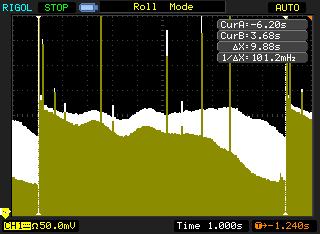
\includegraphics[width=8cm]{Imagenes/Mediciones instrumentos/NewFile1.png}
			\caption{Se\~nales recibidas en CH1 cuando est\'a conectado al generador de se\~ales (en blanco) y cu\'ando se carga con la punta X10 (en verde).} \label{img001}
		\end{figure}
			
		Como era de esperar al cargar el nodo con la punta X10, el ancho de banda disminuye considerablemente. Aproximadamente la frecuencia de corte observada en la Figura es $$f_{-3dB}=245MHz$$
		En la Figura \ref{img000} se vizualizan las se\~n ales que toman CH1 y CH2. La se\~nal del CH1 es la misma que en el caso anterior con el ancho de banda reducido por el efecto de carga generado por la punta X10. Por otra parte la se\~nal del CH2 presenta un sobrepico en altas frecuencias en lugar de actuar como un sistema de primer orden.
		\begin{figure}[!htb]
			\centering
			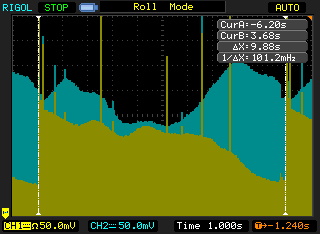
\includegraphics[width=8cm]{Imagenes/Mediciones instrumentos/NewFile0.png}
			\caption{Se\~nales del CH1 (en verde) y del canal CH2 (en celeste).} \label{img000}
		\end{figure}
									
		\subsection{Punta de prueba X1}
		Se realiza la misma experiencia que en el caso anterior, excepto que ahora el barrido de frecuencias es de $1MHz$ a $21MHz$ y la punta que se conecta al CH2 es X1. Dado que la punta X1 posee una capacitancia equivalente mayor que la punta X10, es esperable que el ancho de banda de la se\~nal se reduzca en mayor medida.

		En la Figura \ref{img003}, se pueden ver las se\~nales del CH1 antes y despu\'es de cargarlo con la punta del CH2. 
		\begin{figure}[!htb]
			\centering
			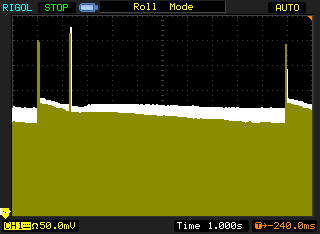
\includegraphics[width=8cm]{Imagenes/Mediciones instrumentos/NewFile4.png}
			\caption{Se\~nales del CH1 cuando est\'a conectada al generador (en blanco) y cuando se carga con la punta X1(en verde).} \label{img003}
		\end{figure}
		
		Por otra parte en la Figura \ref{img002}, se pueden ver las se\~nales que proviene del CH1 y el CH2
		La frecuencia de corte observada en la Figura es $$f_{-3dB}=9MHz$$
		\begin{figure}[!htb]
			\centering
			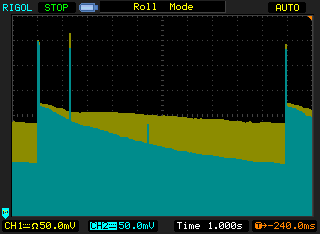
\includegraphics[width=8cm]{Imagenes/Mediciones instrumentos/NewFile3.png}
			\caption{Se\~nales del CH1 (en verde) y del canal CH2 (en celeste).} \label{img002}
		\end{figure}						
		
		\subsection{Punta de prueba de corriente}
		En esta secci\'on se comparan los anchos de banda de puntas de corriente de dos fabricantes, Agilent$_{\textregistered}$  y Tetronix$_{\textregistered} )$.
		El procedimiento es similar al realizado en las experiencias previas. Se utiliza un generador de se\~nales que barre frecuencias desde $300KHz$ a $30MHz$ en un tiempo aproximado de $10s$, la corriente que circula por el coaxil que se conecta al generador es sensada por las puntas de corriente (2 por cada fabricante). En la Figura \ref{img004} y \ref{img005}, se muestran los gr\'aficos obtenidos para las puntas de Agilent$_{\textregistered}$. Los ancho de banda obtenidos de los gr\'aficos, son respectivamente $$f_{-3dB}=15.6MHz$$ y $$f_{-3dB}=9.5MHz$$
		\begin{figure}[!htb]
			\centering
			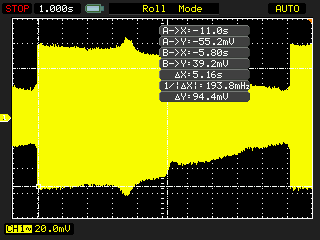
\includegraphics[width=8cm]{Imagenes/Mediciones instrumentos/NewFile5.png}
			\caption{Barrido en frecuencia para una punta de Agilent$_{\textregistered}$.} \label{img004}
		\end{figure}
		
		\begin{figure}[!htb]
			\centering
			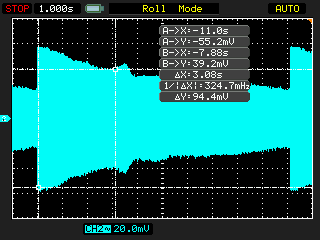
\includegraphics[width=8cm]{Imagenes/Mediciones instrumentos/NewFile6.png}
			\caption{Barrido en frecuencia para una punta de Agilent$_{\textregistered}$.} \label{img005}
		\end{figure}				
		
		Por otra parte, dado que las puntas de corriente de  Tektronix$_{\textregistered} )$ tienen menor ancho de banda se modific\'o el rango de barrido del generador a $300kHz$ a $10MHz$.En las Figuras \ref{img006} y \ref{img007}, se muestran los gr\'aficos obtenidos. De ellos se puede calcular el ancho de banda de cada punta
		$$f_{-3dB}=2.4MHz$$ y $$f_{-3dB}=1.9MHz$$
		\begin{figure}[!htb]
			\centering
			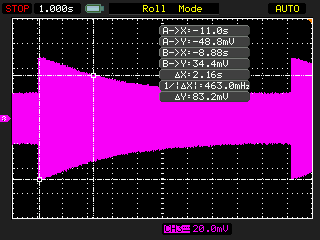
\includegraphics[width=8cm]{Imagenes/Mediciones instrumentos/NewFile7.png}
			\caption{Barrido en frecuencia para una punta de Tektronix$_{\textregistered}$.} \label{img006}
		\end{figure}		
	
		\begin{figure}[!htb]
			\centering
			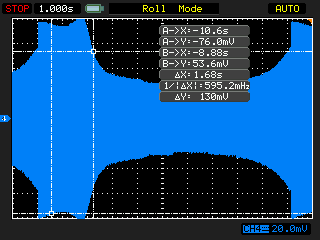
\includegraphics[width=8cm]{Imagenes/Mediciones instrumentos/NewFile8.png}
			\caption{Barrido en frecuencia para una punta de Tektronix$_{\textregistered}$.} \label{img007}
		\end{figure}
		
		\subsection{Tiempo de crecimiento del generador}
		\begin{figure}[!htb]
			\centering
			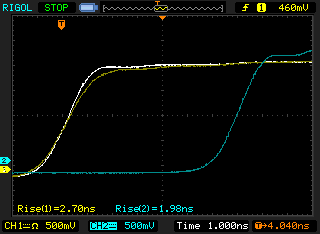
\includegraphics[width=8cm]{Imagenes/Mediciones instrumentos/NewFile10.png}
			\caption{Se\~nales del CH1 (en verde) y del canal CH2 (en celeste)} \label{img008}
		\end{figure}
		
	\section{Conclusiones}
\end{document}

